\documentclass[]{book}
\usepackage{lmodern}
\usepackage{amssymb,amsmath}
\usepackage{ifxetex,ifluatex}
\usepackage{fixltx2e} % provides \textsubscript
\ifnum 0\ifxetex 1\fi\ifluatex 1\fi=0 % if pdftex
  \usepackage[T1]{fontenc}
  \usepackage[utf8]{inputenc}
\else % if luatex or xelatex
  \ifxetex
    \usepackage{mathspec}
  \else
    \usepackage{fontspec}
  \fi
  \defaultfontfeatures{Ligatures=TeX,Scale=MatchLowercase}
\fi
% use upquote if available, for straight quotes in verbatim environments
\IfFileExists{upquote.sty}{\usepackage{upquote}}{}
% use microtype if available
\IfFileExists{microtype.sty}{%
\usepackage{microtype}
\UseMicrotypeSet[protrusion]{basicmath} % disable protrusion for tt fonts
}{}
\usepackage[b5paper,tmargin=1.5cm,bmargin=1.5cm,lmargin=1.5cm,rmargin=1.5cm]{geometry}
\usepackage{hyperref}
\PassOptionsToPackage{usenames,dvipsnames}{color} % color is loaded by hyperref
\hypersetup{unicode=true,
            pdftitle={Intelligent Transportation Systems ITS - II},
            pdfauthor={Andres Ladino - Angelo Furno},
            colorlinks=true,
            linkcolor=Maroon,
            citecolor=Blue,
            urlcolor=Blue,
            breaklinks=true}
\urlstyle{same}  % don't use monospace font for urls
\usepackage{color}
\usepackage{fancyvrb}
\newcommand{\VerbBar}{|}
\newcommand{\VERB}{\Verb[commandchars=\\\{\}]}
\DefineVerbatimEnvironment{Highlighting}{Verbatim}{commandchars=\\\{\}}
% Add ',fontsize=\small' for more characters per line
\usepackage{framed}
\definecolor{shadecolor}{RGB}{248,248,248}
\newenvironment{Shaded}{\begin{snugshade}}{\end{snugshade}}
\newcommand{\AlertTok}[1]{\textcolor[rgb]{0.94,0.16,0.16}{#1}}
\newcommand{\AnnotationTok}[1]{\textcolor[rgb]{0.56,0.35,0.01}{\textbf{\textit{#1}}}}
\newcommand{\AttributeTok}[1]{\textcolor[rgb]{0.77,0.63,0.00}{#1}}
\newcommand{\BaseNTok}[1]{\textcolor[rgb]{0.00,0.00,0.81}{#1}}
\newcommand{\BuiltInTok}[1]{#1}
\newcommand{\CharTok}[1]{\textcolor[rgb]{0.31,0.60,0.02}{#1}}
\newcommand{\CommentTok}[1]{\textcolor[rgb]{0.56,0.35,0.01}{\textit{#1}}}
\newcommand{\CommentVarTok}[1]{\textcolor[rgb]{0.56,0.35,0.01}{\textbf{\textit{#1}}}}
\newcommand{\ConstantTok}[1]{\textcolor[rgb]{0.00,0.00,0.00}{#1}}
\newcommand{\ControlFlowTok}[1]{\textcolor[rgb]{0.13,0.29,0.53}{\textbf{#1}}}
\newcommand{\DataTypeTok}[1]{\textcolor[rgb]{0.13,0.29,0.53}{#1}}
\newcommand{\DecValTok}[1]{\textcolor[rgb]{0.00,0.00,0.81}{#1}}
\newcommand{\DocumentationTok}[1]{\textcolor[rgb]{0.56,0.35,0.01}{\textbf{\textit{#1}}}}
\newcommand{\ErrorTok}[1]{\textcolor[rgb]{0.64,0.00,0.00}{\textbf{#1}}}
\newcommand{\ExtensionTok}[1]{#1}
\newcommand{\FloatTok}[1]{\textcolor[rgb]{0.00,0.00,0.81}{#1}}
\newcommand{\FunctionTok}[1]{\textcolor[rgb]{0.00,0.00,0.00}{#1}}
\newcommand{\ImportTok}[1]{#1}
\newcommand{\InformationTok}[1]{\textcolor[rgb]{0.56,0.35,0.01}{\textbf{\textit{#1}}}}
\newcommand{\KeywordTok}[1]{\textcolor[rgb]{0.13,0.29,0.53}{\textbf{#1}}}
\newcommand{\NormalTok}[1]{#1}
\newcommand{\OperatorTok}[1]{\textcolor[rgb]{0.81,0.36,0.00}{\textbf{#1}}}
\newcommand{\OtherTok}[1]{\textcolor[rgb]{0.56,0.35,0.01}{#1}}
\newcommand{\PreprocessorTok}[1]{\textcolor[rgb]{0.56,0.35,0.01}{\textit{#1}}}
\newcommand{\RegionMarkerTok}[1]{#1}
\newcommand{\SpecialCharTok}[1]{\textcolor[rgb]{0.00,0.00,0.00}{#1}}
\newcommand{\SpecialStringTok}[1]{\textcolor[rgb]{0.31,0.60,0.02}{#1}}
\newcommand{\StringTok}[1]{\textcolor[rgb]{0.31,0.60,0.02}{#1}}
\newcommand{\VariableTok}[1]{\textcolor[rgb]{0.00,0.00,0.00}{#1}}
\newcommand{\VerbatimStringTok}[1]{\textcolor[rgb]{0.31,0.60,0.02}{#1}}
\newcommand{\WarningTok}[1]{\textcolor[rgb]{0.56,0.35,0.01}{\textbf{\textit{#1}}}}
\usepackage{longtable,booktabs}
\usepackage{graphicx,grffile}
\makeatletter
\def\maxwidth{\ifdim\Gin@nat@width>\linewidth\linewidth\else\Gin@nat@width\fi}
\def\maxheight{\ifdim\Gin@nat@height>\textheight\textheight\else\Gin@nat@height\fi}
\makeatother
% Scale images if necessary, so that they will not overflow the page
% margins by default, and it is still possible to overwrite the defaults
% using explicit options in \includegraphics[width, height, ...]{}
\setkeys{Gin}{width=\maxwidth,height=\maxheight,keepaspectratio}
\IfFileExists{parskip.sty}{%
\usepackage{parskip}
}{% else
\setlength{\parindent}{0pt}
\setlength{\parskip}{6pt plus 2pt minus 1pt}
}
\setlength{\emergencystretch}{3em}  % prevent overfull lines
\providecommand{\tightlist}{%
  \setlength{\itemsep}{0pt}\setlength{\parskip}{0pt}}
\setcounter{secnumdepth}{5}
% Redefines (sub)paragraphs to behave more like sections
\ifx\paragraph\undefined\else
\let\oldparagraph\paragraph
\renewcommand{\paragraph}[1]{\oldparagraph{#1}\mbox{}}
\fi
\ifx\subparagraph\undefined\else
\let\oldsubparagraph\subparagraph
\renewcommand{\subparagraph}[1]{\oldsubparagraph{#1}\mbox{}}
\fi

%%% Use protect on footnotes to avoid problems with footnotes in titles
\let\rmarkdownfootnote\footnote%
\def\footnote{\protect\rmarkdownfootnote}

%%% Change title format to be more compact
\usepackage{titling}

% Create subtitle command for use in maketitle
\newcommand{\subtitle}[1]{
  \posttitle{
    \begin{center}\large#1\end{center}
    }
}

\setlength{\droptitle}{-2em}

  \title{Intelligent Transportation Systems ITS - II}
    \pretitle{\vspace{\droptitle}\centering\huge}
  \posttitle{\par}
    \author{Andres Ladino - Angelo Furno}
    \preauthor{\centering\large\emph}
  \postauthor{\par}
      \predate{\centering\large\emph}
  \postdate{\par}
    \date{29/11/2018}

\usepackage[utf8]{inputenc} % Accent inputs
\usepackage[english]{babel} % English language/hyphenation
\usepackage[T1]{fontenc} % Font encoding
\usepackage{microtype} % Rendering
\usepackage{xspace} % Space optimization
\usepackage{fourier}
\usepackage{booktabs}
\usepackage{amsthm}
\makeatletter
\def\thm@space@setup{%
  \thm@preskip=8pt plus 2pt minus 4pt
  \thm@postskip=\thm@preskip
}
\makeatother

\usepackage{amsthm}
\newtheorem{theorem}{Theorem}[chapter]
\newtheorem{lemma}{Lemma}[chapter]
\theoremstyle{definition}
\newtheorem{definition}{Definition}[chapter]
\newtheorem{corollary}{Corollary}[chapter]
\newtheorem{proposition}{Proposition}[chapter]
\theoremstyle{definition}
\newtheorem{example}{Example}[chapter]
\theoremstyle{definition}
\newtheorem{exercise}{Exercise}[chapter]
\theoremstyle{remark}
\newtheorem*{remark}{Remark}
\newtheorem*{solution}{Solution}
\begin{document}
\maketitle

{
\hypersetup{linkcolor=black}
\setcounter{tocdepth}{1}
\tableofcontents
}
\begin{center}\rule{0.5\linewidth}{\linethickness}\end{center}

\hypertarget{its-for-smart-mobility}{%
\chapter*{ITS for Smart Mobility}\label{its-for-smart-mobility}}
\addcontentsline{toc}{chapter}{ITS for Smart Mobility}




\begin{figure}

{\centering 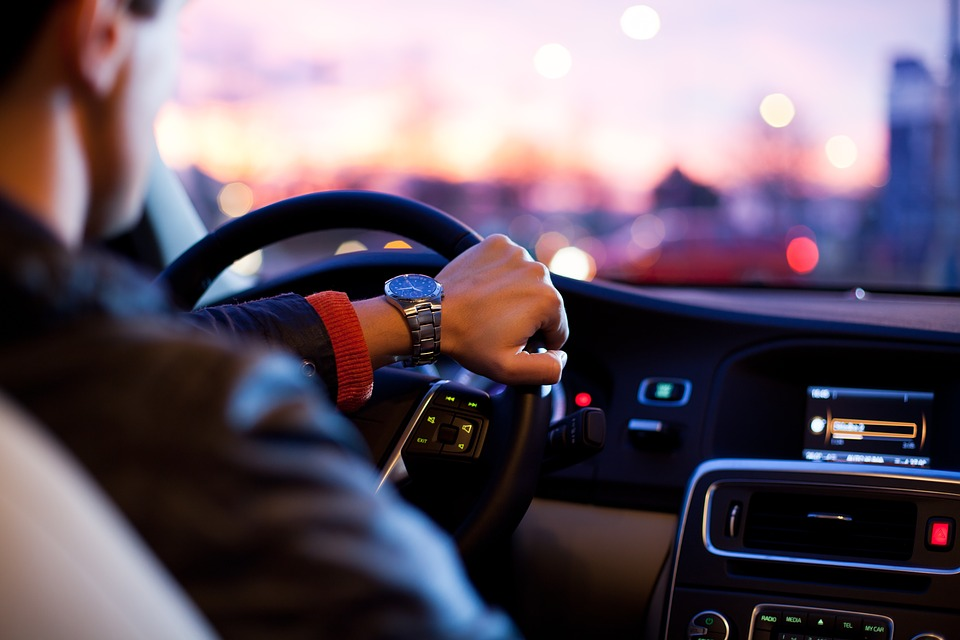
\includegraphics{images/01-car} 

}

\caption{New connected vehicles
\href{Taken\%20from:\%20https://pixabay.com}{https://pixabay.com}.}\label{fig:car}
\end{figure}

\hypertarget{context}{%
\section*{Context}\label{context}}
\addcontentsline{toc}{section}{Context}

Traffic congestion on urban roads is a problem of great interest
nowadays since it strongly affects security and pollution. Workfoce
centralization, population and economic growth alongside with continuous
urbanization are the main causes of traffic congestion. As cities strive
to update/expand the current infrastructures the development of
Information Technologies bring new possiblities as an alternative
solution for transportation systems.

The current project aims to explore some of the new technologies used in
the so called Intelligent Transportation Systems (ITS). They objective
is to study to a certain level of detail some of the new traffic
management systems that will conduct new ways of transportation in the
XXI century. The general idea is based on the fact that information
collected by sensors within traffic networks or in-vehicles sensors can
collect information regarding the traffic condition, perform estimation
of unknown traffic states and decide on specific actions to modify this
state.

\begin{center}\rule{0.5\linewidth}{\linethickness}\end{center}

\hypertarget{projects}{%
\section*{Projects}\label{projects}}
\addcontentsline{toc}{section}{Projects}

Specially, in this case the project will be focused in four main
activities:

\begin{itemize}
\tightlist
\item
  \textbf{Trafic signal design:} This projects aims to study how to
  optimally deal with the design of light cycles to optimize the traffic
  performance. Based on information collected by infrastructure based
  sensors the traffic state can be determined and specific decisions in
  terms on green/red light times can be dynamically adapted.
\item
  \textbf{Vehicle Platooning:} New in-vechicle sensors create situations
  in which vehicles may exchange information to improve traffic
  conditions. This project aims to study control algorithms implemented
  in the V2V (Vehicle-vehicle) communication layer that can be used to
  design traffic decisions.
\item
  \textbf{Density reconstruction:} Sensors installed in traffic
  infrastructures provide information regarding the traffic state.
  Nevertheless the solution is not scalable to cover large cities due to
  the economical leverage required to deploy this technology. Algorithms
  to reconstruct traffic information may provide a promising future for
  accurately determine the traffic state of a city. The aim of this
  project is to study how multiple sources of information can be
  integrated to reconstruct traffic variables within a city.
\end{itemize}

\begin{center}\rule{0.5\linewidth}{\linethickness}\end{center}

\hypertarget{general-objectives}{%
\section*{General Objectives}\label{general-objectives}}
\addcontentsline{toc}{section}{General Objectives}

\begin{itemize}
\tightlist
\item
  Identify new technologies implemented in the Intelligent Transporation
  Systems and investigate how these technologies are deployed in real
  systems.
\item
  Define and determine adequate models that are suitable for deploying
  new ITS technologies.
\item
  Develop specific solutions for ITS that can be tested under
  pre-defined scenarios.
\end{itemize}

\hypertarget{project-information}{%
\chapter*{Project information}\label{project-information}}
\addcontentsline{toc}{chapter}{Project information}

\hypertarget{deliverables}{%
\section*{Deliverables}\label{deliverables}}
\addcontentsline{toc}{section}{Deliverables}

The project is mainly composed in 3 phases.

\begin{enumerate}
\def\labelenumi{\arabic{enumi}.}
\item
  \textbf{Problem identification \& literature review:} This phases
  consists in:

  \begin{enumerate}
  \def\labelenumii{\arabic{enumii}.}
  \item
    Identify particularly the problem under study, meaning the system to
    be controlled and the way it is assesed.
  \item
    Retrieve bibliographical information about the problem under study.
  \item
    Summarize the already proposed alternatives in the existing
    literature.
  \end{enumerate}

  The main objective of this phase is to understand what are the main
  challenges when solving the specific project under study and to
  present in general ways how this problem has been solved.
\item
  \textbf{Setting up a suitable model:} Once the problem has been
  identified the main objective is to precisely describe the traffic
  models that are suitable for the approach. For this phase the stages
  are divided as:

  \begin{enumerate}
  \def\labelenumii{\arabic{enumii}.}
  \tightlist
  \item
    Determine a specific traffic model that can be used for the
    corresponding situation
  \item
    Define the scenario in which the solution should be tested
  \item
    Pre establish parameters and requirements for the solution to be
    implemented.
  \end{enumerate}
\item
  \textbf{Experimental results:} Finally, the main objective is to
  perform a validation and solution for the problem under study. Several
  tools are provided for this purpose like micro/macro
\end{enumerate}

\begin{center}\rule{0.5\linewidth}{\linethickness}\end{center}

\hypertarget{reporting}{%
\section*{Reporting}\label{reporting}}
\addcontentsline{toc}{section}{Reporting}

In order to fullfill the requirements for each phase each group should
provide a report as follows:

\begin{itemize}
\item
  \emph{Report 1:} Summarizes the results of the 1. Problem
  identification \& literature review and 2. Setting up a suitable
  model. (\textbf{\emph{Due date: January 9th, 2018}})
\item
  \emph{Report 2:} Summarizes the results of the phase 3.Experimental
  results (\textbf{\emph{Due date: January 23rd, 2019}})
\end{itemize}

\hypertarget{project-1-signalized-traffic}{%
\chapter*{Project 1: Signalized
Traffic}\label{project-1-signalized-traffic}}
\addcontentsline{toc}{chapter}{Project 1: Signalized Traffic}

The main objective of this project is to design \emph{traffic light
signal} controls in order to optimize particular traffic conditions.
Traffic signals regularly pre-establish fixed values \emph{red} or
\emph{green} for a particular intersection. In fact the behavior can be
modeled as:



\begin{figure}

{\centering 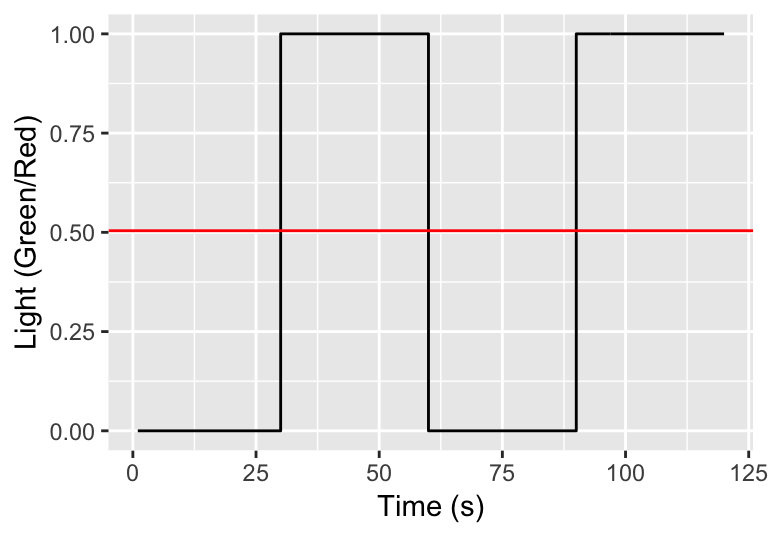
\includegraphics{its-2-project_files/figure-latex/tlight-1} 

}

\caption{Traffic light signal example.}\label{fig:tlight}
\end{figure}

The relationship between the switched green/red time in a traffic light
can be represented by a pulse signal (Figure \ref{fig:tlight}). The red
line in the figure represents the \emph{duty cycle} which represents the
fraction of time the light was in green (\(1\)) with respect to the
total cycle time (\(60s\)). In this case, the main objective is to study
traffic models that can model signalized intersections and design
control laws.

\begin{center}\rule{0.5\linewidth}{\linethickness}\end{center}

\hypertarget{objectives}{%
\section*{Objectives}\label{objectives}}
\addcontentsline{toc}{section}{Objectives}

The main objective of this project is to:

\begin{enumerate}
\def\labelenumi{\arabic{enumi}.}
\tightlist
\item
  Study the fundamental aspects of traffic signal control strategies.
\item
  Obtain and simulate a macroscopic traffic model for a urban network
  with traffic signals
\item
  Create and design control strategies applied via traffic signals in
  urban traffic networks.
\item
  Compare the behavior of fixed-time traffic signal polices and
  dynamic-time traffic signal polices.
\end{enumerate}

\hypertarget{description}{%
\section*{Description}\label{description}}
\addcontentsline{toc}{section}{Description}

\hypertarget{task-1-modeling}{%
\subsection*{Task 1: Modeling}\label{task-1-modeling}}
\addcontentsline{toc}{subsection}{Task 1: Modeling}

Check models for macroscopic networks: (Grandinetti, Canudas-de-wit, and
Garin \protect\hyperlink{ref-Grandinetti2015}{2015}), (Grandinetti,
Garin, and Canudas-de-wit
\protect\hyperlink{ref-Grandinetti2016}{2015}),(Varaiya
\protect\hyperlink{ref-Varaiya2013:TR-C}{2013}). Determine the
parameters required to model a road traffic network.

\hypertarget{context-1}{%
\subsubsection*{Context}\label{context-1}}
\addcontentsline{toc}{subsubsection}{Context}

Before implementing a real scenario in this phase we aim to describe the
context of a virtual example. Consider the following traffic urban
corridor which obeys a simplified version of the real arterial scenario.



\begin{figure}

{\centering 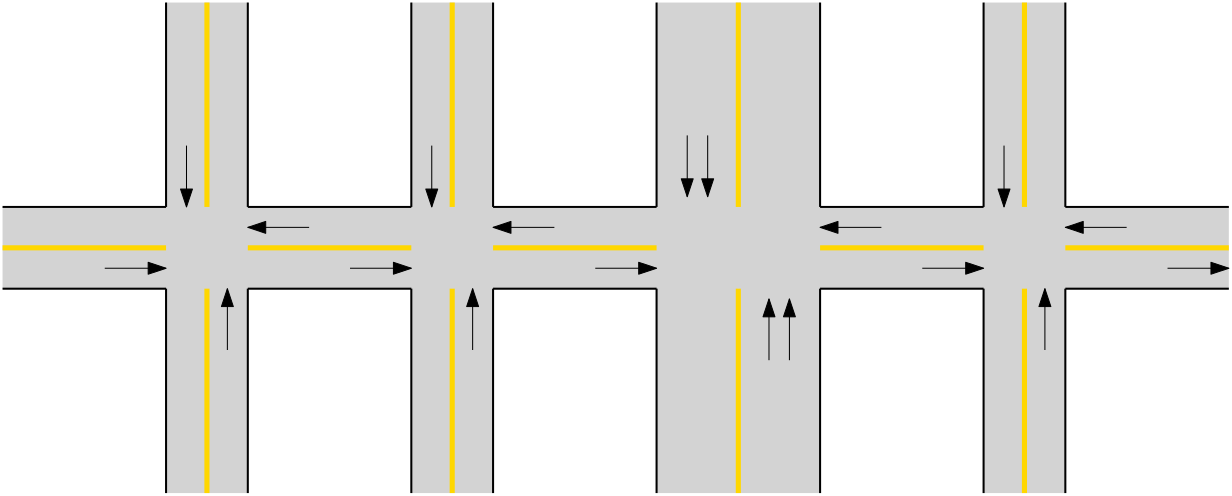
\includegraphics{images/p1-01-network} 

}

\caption{Example of traffic network.}\label{fig:city}
\end{figure}

The network of Figure \ref{fig:city} represents a regular corridor in a
city like. The priority for this type of corridors is to maximize the
priority of green time so the traffic does not get congested along the
network. It is important to highlight that for the proposed network

\hypertarget{questions}{%
\subsubsection*{Questions}\label{questions}}
\addcontentsline{toc}{subsubsection}{Questions}

\begin{itemize}
\tightlist
\item
  Based on a literature review, determine current existing traffic
  models for signalized traffic networks.
\item
  For the network in Figure \ref{fig:city}, build a macroscopic
  signalized traffic model.
\item
  Determine the \emph{signalized/averaged} traffic model for the case
  where lights are installed along each intersection of the corridor.
  For those roads in which direction is not explicitly defined, consider
  the direction of a regular intersection.
\end{itemize}

\hypertarget{expected-outcomes}{%
\subsubsection*{Expected outcomes}\label{expected-outcomes}}
\addcontentsline{toc}{subsubsection}{Expected outcomes}

\begin{itemize}
\item
  Present a brief summary of the existing current models for signalized
  traffic networks. At same time highlight the key features of these
  models and the remaining difficulties. Consider including references
  for the presented models.
\item
  Based on (Grandinetti, Canudas-de-wit, and Garin
  \protect\hyperlink{ref-Grandinetti2015}{2015}) obtain a model for the
  signalized network of Figure \ref{fig:city} and the parameters
  required model this corridor.
\item
  Define the set of parameters for the traffic network, notably those
  related to the fundamental diagram as well as the traffic light signal
  timings. Consider a fixed setup of this parameters for the moment and
  overall explain the reason of the choice.
\end{itemize}

\begin{center}\rule{0.5\linewidth}{\linethickness}\end{center}

\hypertarget{task-2-simulation}{%
\subsection*{Task 2: Simulation}\label{task-2-simulation}}
\addcontentsline{toc}{subsection}{Task 2: Simulation}

Dynamic simulation of open loop traffic networks. For this task be sure
to review already implemented simulations available at
\href{https://github.com/andres-ladino-ifsttar/traffic-macrosimulator}{Link}.
Get familiar with the code here developed before you enter into details
of implementation.

\hypertarget{context-2}{%
\subsubsection*{Context}\label{context-2}}
\addcontentsline{toc}{subsubsection}{Context}

Based on the model established in the \textbf{Task 1} and considering a
family of specific parameters, perform a simulation for a constant
demand value of demand in \(veh/hr\) as specified in the
Figure\ref{fig:flow}.



\begin{figure}

{\centering 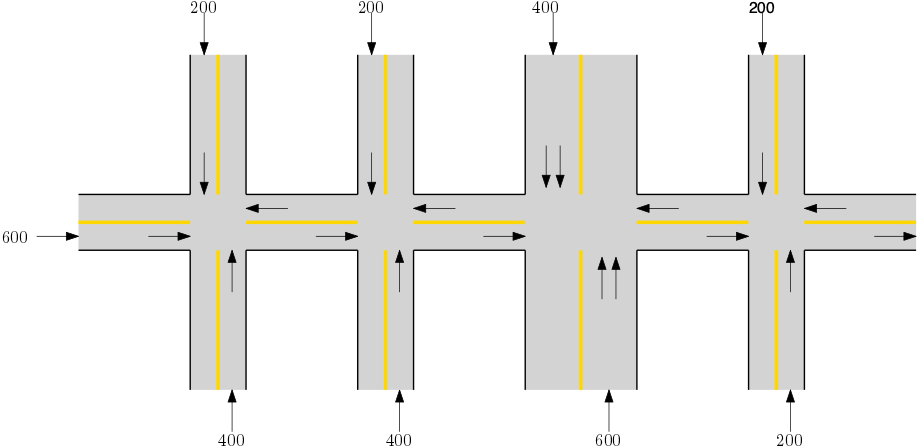
\includegraphics{images/p1-02-flows} 

}

\caption{Demand profiles for a specified scenario.}\label{fig:flow}
\end{figure}

\hypertarget{questions-1}{%
\subsubsection*{Questions}\label{questions-1}}
\addcontentsline{toc}{subsubsection}{Questions}

\begin{itemize}
\item
  Simulate and obtain density plots of the dynamic the behaviour when
  the \emph{duty cyle} of lights is similar for all the traffic lights.
  \(50\%\)
\item
  Does the current values create a congestion in the proposed network?
\item
  How can the performance of the network be improved? Create a second
  set of parameters for the traffic lights \emph{duty cycle}
\item
  For the existing model and according to (Grandinetti, Canudas-de-wit,
  and Garin \protect\hyperlink{ref-Grandinetti2015}{2015}) obtain the
  two different \emph{density} and \emph{flow} dynamic profiles between
  a \emph{switched} signalized traffic model and an \emph{averaged}
  traffic model
\end{itemize}

\hypertarget{expected-outcomes-1}{%
\subsubsection*{Expected outcomes}\label{expected-outcomes-1}}
\addcontentsline{toc}{subsubsection}{Expected outcomes}

\begin{itemize}
\item
  Present the dynamic profiles for density on each one of the roads
  under different setups of traffic lights. The dynamic profiles should
  specify density per road in time
\item
  Provide comparisons between different traffic signalized models and an
  analysis on how this error evolves according to different values of
  demand.
\item
  Specify a second set of parameters for \emph{duty cycle} that could
  improve the performance of the network with respect to the \(50\%\)
  case. Justify the reason of your choice and verify in results the
  desired behavior.
\end{itemize}

\begin{center}\rule{0.5\linewidth}{\linethickness}\end{center}

\hypertarget{task-3-control-strategy}{%
\subsection*{Task 3: Control strategy}\label{task-3-control-strategy}}
\addcontentsline{toc}{subsection}{Task 3: Control strategy}

For this task we aim to consider the \emph{duty cycle} as a control
input variable to regulate the flow within the traffic network. In this
case take into account that the decision variable needs somehow to be
determined dynamically via a control algorithm.

\hypertarget{context-3}{%
\subsubsection*{Context}\label{context-3}}
\addcontentsline{toc}{subsubsection}{Context}

For the Figure \ref{fig:tlight} the average value can be found as:

\begin{equation}
\bar{u} = \frac{1}{T}\int_0^T u(\tau) d\tau \label{eq:avgu}
\end{equation}

As it is illustrated in (Grandinetti, Garin, and Canudas-de-wit
\protect\hyperlink{ref-Grandinetti2016}{2015}), in Eq. \eqref{eq:avgu} is
easier to design a value for \(\bar{u}\) rather than \(u\) due to its
binary character.

\hypertarget{questions-2}{%
\subsubsection*{Questions}\label{questions-2}}
\addcontentsline{toc}{subsubsection}{Questions}

\begin{itemize}
\item
  Explain and construct a block diagram illustrating the control of the
  road traffic network via traffic signals
\item
  Design and present an algorithm that takes decisions for the traffic
  signals based on the state of the network. How would you construct the
  value of \(u\) based on the congestion state of the network.
\item
  Perform simulations of the system under a preestablished manual
  control and compare it to a situation where the control depends on the
  congestion state of the network.
\end{itemize}

\hypertarget{expected-outcomes-2}{%
\subsubsection*{Expected outcomes}\label{expected-outcomes-2}}
\addcontentsline{toc}{subsubsection}{Expected outcomes}

\begin{itemize}
\item
  Present a comparison between the traffic network with signalized
  control and without signalized control.
\item
  Apply the controller over different versions of the model notably
  \emph{averaged} and \emph{switched}
\item
  Compare the open loop situation with the closed loop situation and
  provide conclussions on the control performance.
\end{itemize}

\begin{center}\rule{0.5\linewidth}{\linethickness}\end{center}

\hypertarget{task-4-performance-evaluation}{%
\subsection*{Task 4: Performance
evaluation}\label{task-4-performance-evaluation}}
\addcontentsline{toc}{subsection}{Task 4: Performance evaluation}

Finally in order to compare it is important to determine indicators than
can be designed in order to compare the effects of introducing an
automated control strategy.

\hypertarget{context-4}{%
\subsubsection*{Context}\label{context-4}}
\addcontentsline{toc}{subsubsection}{Context}

Indicators for traffic networks are regularly expressed in terms of the
state of the network, for example the \emph{Service of Demand} (SoD)
measured in terms of flow:

\begin{equation}
SOD = \int_0^T \sum_{r \in R} f_r(\tau) d\tau \label{eq:sod}
\end{equation}

Or the \emph{Total Travel Distance} (TTD) measured in terms of the
density

\begin{equation}
TTD = \int_0^T \sum_{r \in R} \rho_r(\tau) d\tau \label{eq:ttd}
\end{equation}

\hypertarget{questions-3}{%
\subsubsection*{Questions}\label{questions-3}}
\addcontentsline{toc}{subsubsection}{Questions}

\begin{itemize}
\item
  What does the aforementioned indicators represent?
\item
  Measure the indicators over the traffic network with a manual setup of
  traffic signals \emph{open-loop} vs a controlled setup of traffic
  signals \emph{closed-loop}.
\end{itemize}

\hypertarget{expected-outcomes-3}{%
\subsubsection*{Expected outcomes}\label{expected-outcomes-3}}
\addcontentsline{toc}{subsubsection}{Expected outcomes}

\begin{itemize}
\item
  Report indicators for both cases and conclude about the results.
\item
  Provide recomendations on how to design \(u\) for the corridor
\end{itemize}

\hypertarget{sources}{%
\section*{Sources}\label{sources}}
\addcontentsline{toc}{section}{Sources}

For more details on how to deploy traffic simulations and traffic models
please check:

\begin{itemize}
\item
  \href{https://github.com/andres-ladino-ifsttar/traffic-macrosimulator}{Traffic
  Macrosimulator - Github}
\item
  For traffic models check (Grandinetti, Canudas-de-wit, and Garin
  \protect\hyperlink{ref-Grandinetti2015}{2015}) available
  \href{https://hal.archives-ouvertes.fr/hal-01188535}{Link} and
  (Grandinetti, Garin, and Canudas-de-wit
  \protect\hyperlink{ref-Grandinetti2016}{2015}) available at
  \href{https://hal.archives-ouvertes.fr/hal-01188811}{Link}
\end{itemize}

\hypertarget{project-2-vehicle-platooning}{%
\chapter*{Project 2: Vehicle
Platooning}\label{project-2-vehicle-platooning}}
\addcontentsline{toc}{chapter}{Project 2: Vehicle Platooning}

The main objective of this project is to design a controller for a
platoon of vehicles in order to optimize the traffic flow and reduce the
fuel consumption. A platoon of vehicles can be seen as:



\begin{figure}

{\centering 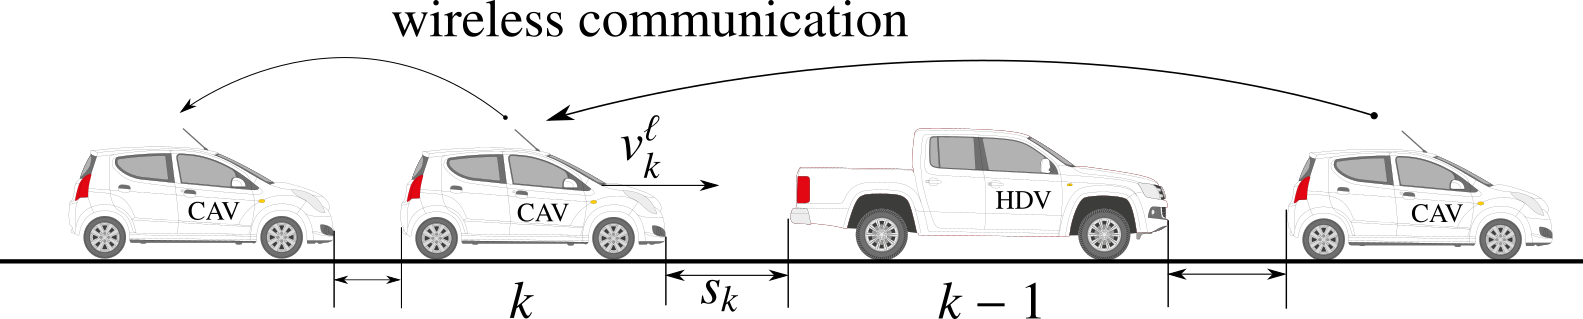
\includegraphics{images/p2-cavs} 

}

\caption{Example of a vehicle platoon.}\label{fig:cav}
\end{figure}

The objective illustrated in Figure \ref{fig:cav} is to control the
\emph{headway space} between two single vehicles in a formation of
multiple vehicles. This project is inspired in works presented on
(Duret, Wang, and Ladino
\protect\hyperlink{ref-Duret2019:ISTTT}{2019}\protect\hyperlink{ref-Duret2019:ISTTT}{a}),
(Wang et al. \protect\hyperlink{ref-Meng2014b:TR-C}{2014}) but more
information about platoons can be found at (Ali, Garcia, and Martinet
\protect\hyperlink{ref-Ali2015:ITSM}{2015}).

\hypertarget{objectives-1}{%
\section*{Objectives}\label{objectives-1}}
\addcontentsline{toc}{section}{Objectives}

The main objective of this project is to:

\begin{enumerate}
\def\labelenumi{\arabic{enumi}.}
\tightlist
\item
  Study and understand the fundamental problem of string stability.
\item
  Obtain and create a dynamic model for vehicle platoons and asociate
  its parameters with traffic theory.
\item
  Create and design a control strategy for the headway space and analyze
  its behavior.
\item
  Compare and analyze the behavior of parameter setups for variations of
  the proposed control strategy
\end{enumerate}

\hypertarget{description-1}{%
\section*{Description}\label{description-1}}
\addcontentsline{toc}{section}{Description}

\hypertarget{task-1-platoon-modeling}{%
\subsection*{Task 1: Platoon modeling}\label{task-1-platoon-modeling}}
\addcontentsline{toc}{subsection}{Task 1: Platoon modeling}

Consider the dynamical model presented in (Duret, Wang, and Ladino
\protect\hyperlink{ref-Duret2019:ISTTT}{2019}\protect\hyperlink{ref-Duret2019:ISTTT}{a}),
(Turri, Besselink, and Johansson
\protect\hyperlink{ref-Turri2017}{2017}) where the problem of truck
platooning is detailed.

\hypertarget{context-5}{%
\subsubsection*{Context}\label{context-5}}
\addcontentsline{toc}{subsubsection}{Context}

In general the platoon problem is a \emph{dynamic control problem} where
the objective is to regulate or mantain the value of a specific variable
within the system at a desired level. In order to produce this
regulation a \emph{controller} is requrired and in most of the cases
cases there is always a way to express the dynamical model in the
following form:

\begin{align}
\dot{x}(t) = f(x(t), u(t)) \label{eq:platoon}
\end{align}

where \(x(t), u(t)\) correspond to the state vector, and the control
vector of the system. In general a system describing this behavior is
called \emph{dynamic} system. In case of platoon the state vector
represents all the variables that contain \emph{minimum} information to
represent the system like, vehicle position, speed, or headway space.
The control vector correspond to the variables that are inputs to the
systems, e.g.~acceleration when modifying the state of a vehicle.

\hypertarget{questions-4}{%
\subsubsection*{Questions}\label{questions-4}}
\addcontentsline{toc}{subsubsection}{Questions}

\begin{itemize}
\tightlist
\item
  What are the main goals of platoon strategies, and how they can
  improve the traffic in future?
\item
  Create a model for a platoon of 4 vehicles that considers a simple
  dynamic model of 2nd order and a 3rd order one. \textbf{Note: Consider
  for this case a model in which no drag is present within the model.}.
  This model can be written as in \eqref{eq:platoon} where the stability
  can be analyzed.
\item
  Which could be the traffic parameters in this kind of models?
\end{itemize}

\hypertarget{expected-outcomes-4}{%
\subsubsection*{Expected outcomes}\label{expected-outcomes-4}}
\addcontentsline{toc}{subsubsection}{Expected outcomes}

\begin{itemize}
\tightlist
\item
  Present a brief summary on the motivations to create vehicle platoons
  and the main existing models that can be developed for this purpose.
\item
  Based on the work of (Duret, Wang, and Ladino
  \protect\hyperlink{ref-Duret2019:ISTTT}{2019}\protect\hyperlink{ref-Duret2019:ISTTT}{a}),
  (Wang et al. \protect\hyperlink{ref-Meng2014b:TR-C}{2014}) determine
  writedown the state equations for a platoon model of 4 vehicles of
  \emph{2nd order} and \emph{3rd order}.\\
\item
  Determine the stability properties of the model. Stability properties
  are associated to the location of zeros and poles of the transfer
  function of the model or eigen values of the matrix
  \href{https://en.wikipedia.org/wiki/Stability_theory}{See more}
\end{itemize}

\begin{center}\rule{0.5\linewidth}{\linethickness}\end{center}

\hypertarget{task-2-open-loop-simulation}{%
\subsection*{Task 2: Open loop
simulation}\label{task-2-open-loop-simulation}}
\addcontentsline{toc}{subsection}{Task 2: Open loop simulation}

\hypertarget{context-6}{%
\subsubsection*{Context}\label{context-6}}
\addcontentsline{toc}{subsubsection}{Context}

One of the first studies in terms of analyzing the properties of a
dynamical system is the dynamical response of the system. This response
can be characterized by the step response of the system to a specific
control input.



\begin{figure}

{\centering 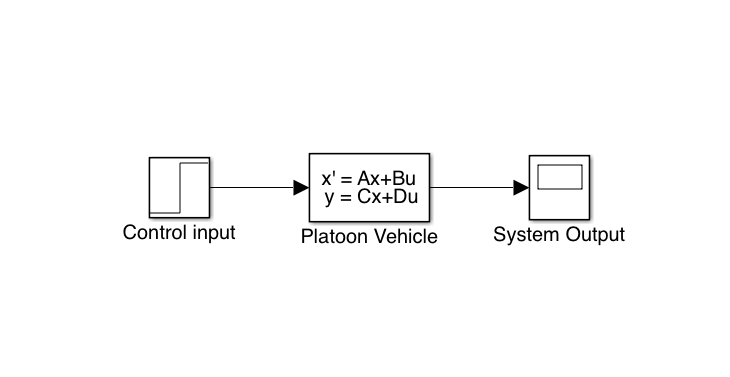
\includegraphics{images/p2-02-control-open} 

}

\caption{Open loop system.}\label{fig:opencav}
\end{figure}

For the case of a platoon vehicle the input in \emph{open} loop are the
accelerations of all vehicles. It seems logical that if a vehicle
modifies its speed from a specific value the space between two vehicles.
We are going to verify this behavior at simulation level.

\hypertarget{questions-5}{%
\subsubsection*{Questions}\label{questions-5}}
\addcontentsline{toc}{subsubsection}{Questions}

\begin{itemize}
\tightlist
\item
  Which is the response of spacing of all vehicles when an impulse of
  deceleration of amplitude \(u = 0.1m/s^2\) is performed over the
  second vehicle? *
\item
  Are there any differences between the spacings when applying the
  decceleration over a \emph{2nd order} model or a \emph{3rd order
  model}?
\item
  Consider the \emph{time engine} constant in the \emph{3rd order}
  model. What is the effect of this vale in the dynamic acceleration/
  decceleration of the system?
\end{itemize}

\hypertarget{expected-outcomes-5}{%
\subsubsection*{Expected outcomes}\label{expected-outcomes-5}}
\addcontentsline{toc}{subsubsection}{Expected outcomes}

\begin{itemize}
\tightlist
\item
  Create a simulation of the \emph{2nd /3rd order} platoon vehicle
  models in which the inputs are the accelerations of all vehicles and
  the outcomes are the headway spaces, and speeds of each vehicle.
\item
  Retrieve the dynamic response of the headway space for the 2nd order/
  3rd order for an impulse of \(u = 0.1m/s^2\)
\item
  Obtain the trajectories in space and time for the platoon of 4
  vehicles.
\end{itemize}

\hypertarget{task-3-vehicle-platoon-control}{%
\subsection*{Task 3: Vehicle platoon
control}\label{task-3-vehicle-platoon-control}}
\addcontentsline{toc}{subsection}{Task 3: Vehicle platoon control}

\begin{center}\rule{0.5\linewidth}{\linethickness}\end{center}

\hypertarget{context-7}{%
\subsubsection*{Context}\label{context-7}}
\addcontentsline{toc}{subsubsection}{Context}

In order to control the system a feedback loop should be introduced in
terms of accelerations of vehicles as shown in the Figure
\ref{fig:closedcav}



\begin{figure}

{\centering 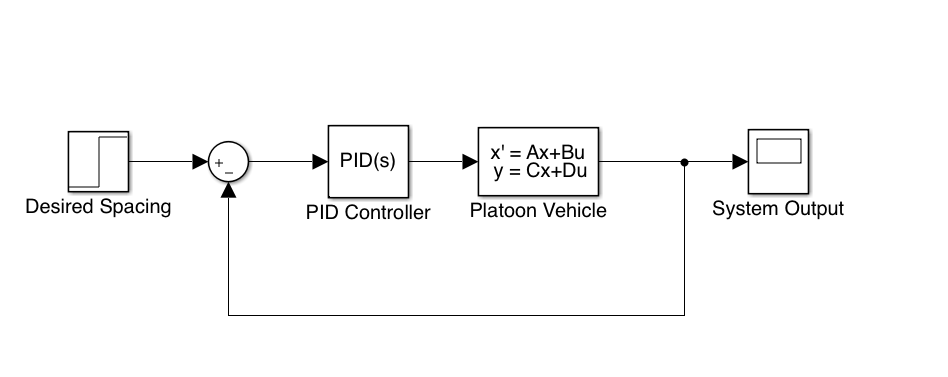
\includegraphics{images/p2-03-closed-loop} 

}

\caption{Closed loop system.}\label{fig:closedcav}
\end{figure}

Whithin the Figure \ref{fig:closedcav} the main objective is to create a
closed loop that provides information in order to take the decision.
These strategies have been already studied in literature. (Wang et al.
\protect\hyperlink{ref-Meng2014b:TR-C}{2014}), (Ali, Garcia, and
Martinet \protect\hyperlink{ref-Ali2015:ITSM}{2015}).

\hypertarget{questions-6}{%
\subsubsection*{Questions}\label{questions-6}}
\addcontentsline{toc}{subsubsection}{Questions}

\begin{itemize}
\tightlist
\item
  Based on the control strategy proposed in (Wang et al.
  \protect\hyperlink{ref-Meng2014b:TR-C}{2014}). Which is one of the
  possibles control structures that can be used for these systems?
\item
  Define and justify some specific values for the proportional integral
  control parameters.
\item
  Set the desire spacing of the system to a specific value of \(10m\)
  for all vehicles, then test a change in the headway space of \(5m\)
  for one of the vehicles. What do you see as a different behavior?
\end{itemize}

\hypertarget{expected-outcomes-6}{%
\subsubsection*{Expected outcomes}\label{expected-outcomes-6}}
\addcontentsline{toc}{subsubsection}{Expected outcomes}

\begin{itemize}
\tightlist
\item
  Provide the dynamical response of the open-loop (headway space/speed)
  system, (all headway spacings/ speed profiles) to a change in
  decceleration of \(0.1m/s^2\), applied over 1s.\\
\item
  Provide the dynamical response of the closed-loop (headway
  space/speed) system, (all headway spacings/ speed profiles) to a
  change in spacing of \(5m\).
\item
  Compare the situations and conclude about the implementation of
  control systems on vehicle automatization. What are the benefits of
  implementing this type of algorithms?
\end{itemize}

\hypertarget{task-4-performance-evaluation-1}{%
\subsection*{Task 4: Performance
evaluation}\label{task-4-performance-evaluation-1}}
\addcontentsline{toc}{subsection}{Task 4: Performance evaluation}

\hypertarget{context-8}{%
\subsubsection*{Context}\label{context-8}}
\addcontentsline{toc}{subsubsection}{Context}

In order to provide a final evaluation it is important to measure the
dynamical performance of the control strategy. This dynamical response
can be measured as in \ref{fig:dynamic2}.



\begin{figure}

{\centering 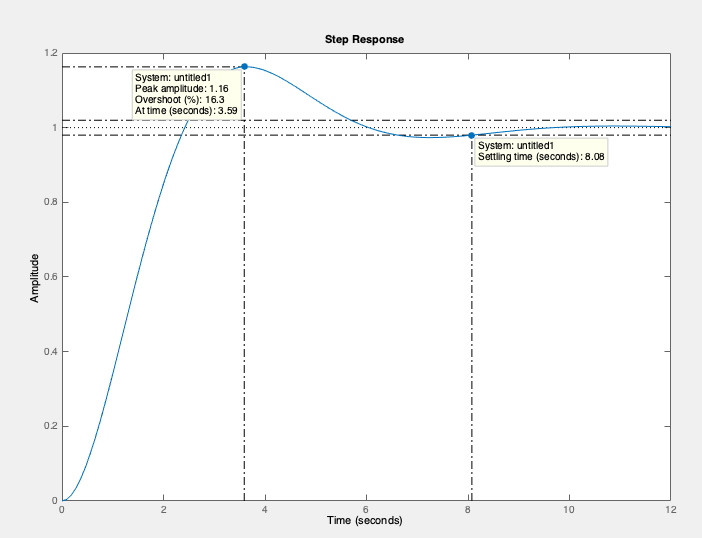
\includegraphics{images/p2-04-evaluation} 

}

\caption{Typical dynamical response for a 2nd order model}\label{fig:dynamic2}
\end{figure}

\hypertarget{questions-7}{%
\subsubsection*{Questions}\label{questions-7}}
\addcontentsline{toc}{subsubsection}{Questions}

\begin{itemize}
\tightlist
\item
  Measure the dynamical response, setting time, rise time for the
  controller operated on the 2nd order model and 3rd order model. What
  can you conclude about the dynamical step response?
\item
  Provide a variation of parameters in the contoller provided. How the
  parameters may affect the stability of the model?
\end{itemize}

\hypertarget{expected-outcomes-7}{%
\subsubsection*{Expected outcomes}\label{expected-outcomes-7}}
\addcontentsline{toc}{subsubsection}{Expected outcomes}

\begin{itemize}
\tightlist
\item
  Provide an analysis from values obtained of simulations of the same
  control for multiple models (2nd/3rd order).
\item
  Construct and determine the effects of modifying control parameters
  when they are applied to multiple models.
\end{itemize}

\hypertarget{sources-1}{%
\section*{Sources}\label{sources-1}}
\addcontentsline{toc}{section}{Sources}

For more details on how to deploy traffic simulations and traffic models
please check:

\begin{itemize}
\item
  \href{https://github.com/research-licit/Hierarchical-Platooning/blob/dev/Operational/platoon-closed-3rd.py}{Simulation
  results - Github}
\item
  Check (Duret, Wang, and Ladino
  \protect\hyperlink{ref-Duret2019}{2019}\protect\hyperlink{ref-Duret2019}{b})
  available \href{http://bit.ly/Hierarchical_ISTTT}{Link}
\end{itemize}

\hypertarget{project-3-density-reconstruction}{%
\chapter*{Project 3: Density
Reconstruction}\label{project-3-density-reconstruction}}
\addcontentsline{toc}{chapter}{Project 3: Density Reconstruction}

The state of congestion of a city is one of the critical. This project
aims to study the reconstruction of traffic variables from different
type of sources. For more information the detail of this work can be
found at (Lovisari, Canudas-de-wit, and Kibangou
\protect\hyperlink{ref-Lovisari2016}{2016}), (Ladino et al.
\protect\hyperlink{ref-Ladino2018}{2018}).

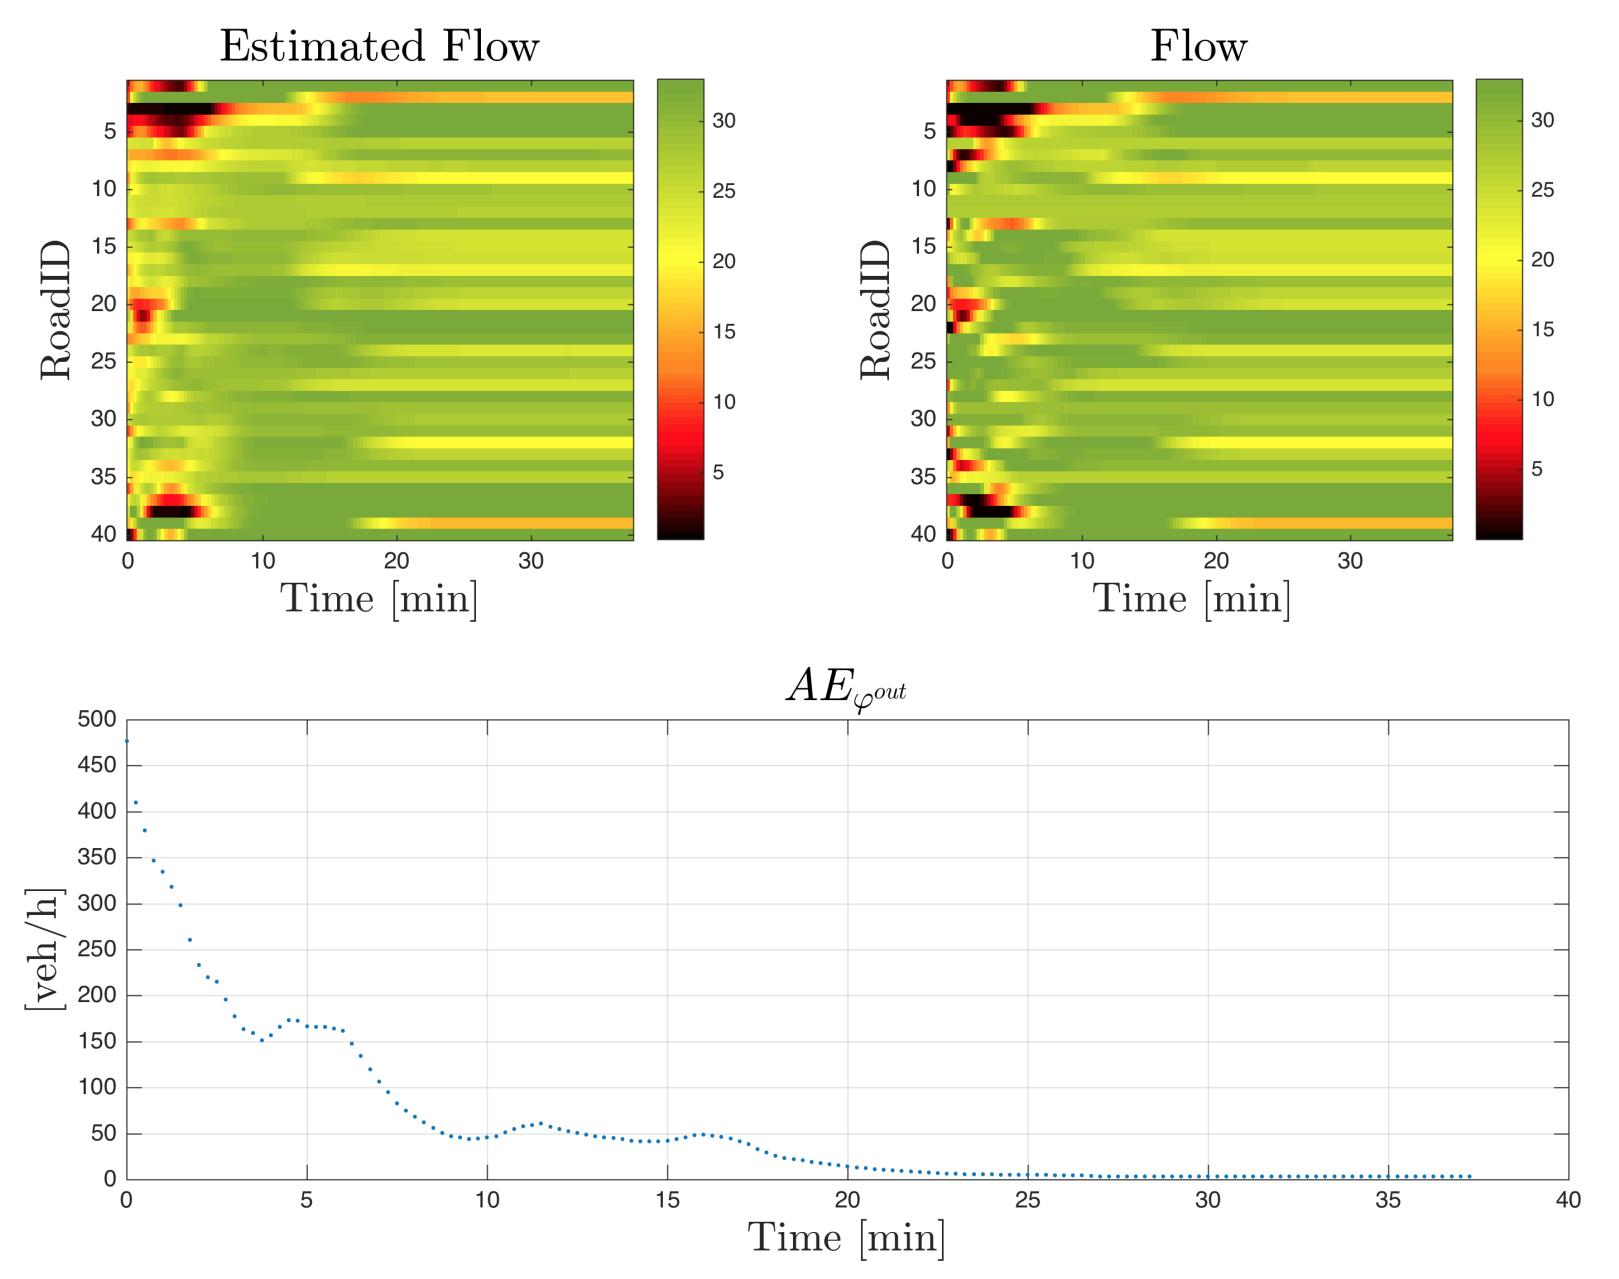
\includegraphics{images/p4-01-density.png}

In this approach in particular, the reconstruction of density will be
based on multiple hypothesys.

\begin{itemize}
\tightlist
\item
  There exist multiple sources of traffic information such as
  \emph{Floating Car Data (FCD)} or \emph{Magnetic Loop Data (MLD)}, the
  nature of these two measurements is different. While FCD can be
  collected easily and almost every where in the traffic network, it is
  not really representative of the congestion state due to the
  penetration rate. Its counter part MLD is accurate when determining
  the amount of vehicles circulating at specific spots, but extending
  this mechanism of measurement to the whole network is expensive.
\item
  The use of models like the LWR model may be useful for providing extra
  information to retrieve the congestion state of the network.
\end{itemize}

\begin{center}\rule{0.5\linewidth}{\linethickness}\end{center}

\hypertarget{objectives-2}{%
\section*{Objectives}\label{objectives-2}}
\addcontentsline{toc}{section}{Objectives}

The main objective of this project is to:

\begin{enumerate}
\def\labelenumi{\arabic{enumi}.}
\tightlist
\item
  Study the LWR model and in particular its network counter part.
\item
  Obtain and simulate a macroscopic traffic model for a urban network.
\item
  Create and design an estimator in order to retrieve the state of the
  network based on heterogenous measurements.
\item
  Compare the behavior and performance of the estimator under multiple
  situations.
\end{enumerate}

\hypertarget{description-2}{%
\section*{Description}\label{description-2}}
\addcontentsline{toc}{section}{Description}

\hypertarget{task-1-modeling-1}{%
\subsection*{Task 1: Modeling}\label{task-1-modeling-1}}
\addcontentsline{toc}{subsection}{Task 1: Modeling}

\hypertarget{context-9}{%
\subsubsection*{Context}\label{context-9}}
\addcontentsline{toc}{subsubsection}{Context}

\hypertarget{questions-8}{%
\subsubsection*{Questions}\label{questions-8}}
\addcontentsline{toc}{subsubsection}{Questions}

\hypertarget{expected-outcomes-8}{%
\subsubsection*{Expected outcomes}\label{expected-outcomes-8}}
\addcontentsline{toc}{subsubsection}{Expected outcomes}

\begin{center}\rule{0.5\linewidth}{\linethickness}\end{center}

\hypertarget{task-2-simulation-1}{%
\subsection*{Task 2: Simulation}\label{task-2-simulation-1}}
\addcontentsline{toc}{subsection}{Task 2: Simulation}

\hypertarget{context-10}{%
\subsubsection*{Context}\label{context-10}}
\addcontentsline{toc}{subsubsection}{Context}

\hypertarget{questions-9}{%
\subsubsection*{Questions}\label{questions-9}}
\addcontentsline{toc}{subsubsection}{Questions}

\hypertarget{expected-outcomes-9}{%
\subsubsection*{Expected outcomes}\label{expected-outcomes-9}}
\addcontentsline{toc}{subsubsection}{Expected outcomes}

\begin{center}\rule{0.5\linewidth}{\linethickness}\end{center}

\hypertarget{task-3-estimation-algorithm}{%
\subsection*{Task 3: Estimation
algorithm}\label{task-3-estimation-algorithm}}
\addcontentsline{toc}{subsection}{Task 3: Estimation algorithm}

\hypertarget{context-11}{%
\subsubsection*{Context}\label{context-11}}
\addcontentsline{toc}{subsubsection}{Context}

\hypertarget{questions-10}{%
\subsubsection*{Questions}\label{questions-10}}
\addcontentsline{toc}{subsubsection}{Questions}

\hypertarget{expected-outcomes-10}{%
\subsubsection*{Expected outcomes}\label{expected-outcomes-10}}
\addcontentsline{toc}{subsubsection}{Expected outcomes}

\begin{center}\rule{0.5\linewidth}{\linethickness}\end{center}

\hypertarget{task-4-estimation-performance}{%
\subsection*{Task 4: Estimation
performance}\label{task-4-estimation-performance}}
\addcontentsline{toc}{subsection}{Task 4: Estimation performance}

\hypertarget{context-12}{%
\subsubsection*{Context}\label{context-12}}
\addcontentsline{toc}{subsubsection}{Context}

\hypertarget{questions-11}{%
\subsubsection*{Questions}\label{questions-11}}
\addcontentsline{toc}{subsubsection}{Questions}

\hypertarget{expected-outcomes-11}{%
\subsubsection*{Expected outcomes}\label{expected-outcomes-11}}
\addcontentsline{toc}{subsubsection}{Expected outcomes}




\begin{Shaded}
\begin{Highlighting}[]
\KeywordTok{plot}\NormalTok{(cars)  }\CommentTok{# a scatterplot}
\end{Highlighting}
\end{Shaded}

\begin{figure}
\centering
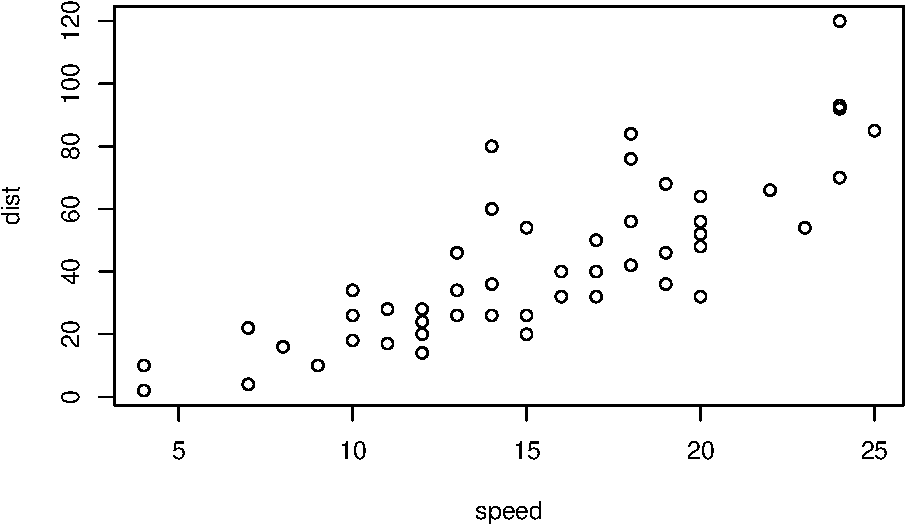
\includegraphics{its-2-project_files/figure-latex/foo-1.pdf}
\caption{\label{fig:foo}A scatterplot of the data \texttt{cars} using \textbf{base} R
graphics.}
\end{figure}

\begin{equation}
f\left(k\right)=\binom{n}{k}p^k\left(1-p\right)^{n-k} \label{eq:binom}
\end{equation}

In \eqref{eq:binom}

Below is an \texttt{align} environment \eqref{eq:align}:

\begin{Shaded}
\begin{Highlighting}[]
\KeywordTok{\textbackslash{}begin}\NormalTok{\{}\ExtensionTok{align}\NormalTok{\}}\SpecialStringTok{ }
\SpecialStringTok{g(X_\{n\}) &= g(}\SpecialCharTok{\textbackslash{}theta}\SpecialStringTok{)+g'(\{}\SpecialCharTok{\textbackslash{}tilde}\SpecialStringTok{\{}\SpecialCharTok{\textbackslash{}theta}\SpecialStringTok{\}\})(X_\{n\}-}\SpecialCharTok{\textbackslash{}theta}\SpecialStringTok{) }\SpecialCharTok{\textbackslash{}notag}\SpecialStringTok{ }\SpecialCharTok{\textbackslash{}\textbackslash{}}
\SpecialCharTok{\textbackslash{}sqrt}\SpecialStringTok{\{n\}[g(X_\{n\})-g(}\SpecialCharTok{\textbackslash{}theta}\SpecialStringTok{)] &= g'}\SpecialCharTok{\textbackslash{}left}\SpecialStringTok{(\{}\SpecialCharTok{\textbackslash{}tilde}\SpecialStringTok{\{}\SpecialCharTok{\textbackslash{}theta}\SpecialStringTok{\}\}}\SpecialCharTok{\textbackslash{}right}\SpecialStringTok{)}
\SpecialStringTok{  }\SpecialCharTok{\textbackslash{}sqrt}\SpecialStringTok{\{n\}[X_\{n\}-}\SpecialCharTok{\textbackslash{}theta}\SpecialStringTok{ ] (}\SpecialCharTok{\textbackslash{}#}\SpecialStringTok{eq:align)}
\KeywordTok{\textbackslash{}end}\NormalTok{\{}\ExtensionTok{align}\NormalTok{\} }
\end{Highlighting}
\end{Shaded}

\begin{align}
g(X_{n}) &= g(\theta)+g'({\tilde{\theta}})(X_{n}-\theta)\\
\sqrt{n}[g(X_{n})-g(\theta)] &= g'\left({\tilde{\theta}}\right)
  \sqrt{n}[X_{n}-\theta ] \label{eq:align}
\end{align}

\hypertarget{sources-2}{%
\section*{Sources}\label{sources-2}}
\addcontentsline{toc}{section}{Sources}

For more details on the project please check:

\begin{itemize}
\item
  \href{https://github.com/aladinoster/density-reconstruction}{Simulation
  results - Github}
\item
  Check (Ladino et al. \protect\hyperlink{ref-Ladino2018}{2018})
  available \href{https://hal.archives-ouvertes.fr/hal-01731356}{Link}
  and (Lovisari, Canudas-de-wit, and Kibangou
  \protect\hyperlink{ref-Lovisari2016}{2016})
  \href{https://hal.archives-ouvertes.fr/hal-01375928}{Link}
\end{itemize}

\hypertarget{reference}{%
\section*{Reference}\label{reference}}
\addcontentsline{toc}{section}{Reference}

The main reference for this project is (Ladino et al.
\protect\hyperlink{ref-Ladino2018}{2018})

\hypertarget{refs}{}
\leavevmode\hypertarget{ref-Ali2015:ITSM}{}%
Ali, Alan, Gaetan Garcia, and Philippe Martinet. 2015. ``The flatbed
platoon towing model for safe and dense platooning on highways.''
\emph{IEEE Intelligent Transportation Systems Magazine} 7 (1): 58--68.
\url{https://doi.org/10.1109/MITS.2014.2328670}.

\leavevmode\hypertarget{ref-Duret2019:ISTTT}{}%
Duret, Aurelien, Meng Wang, and Andres Ladino. 2019a. ``A Hierarchical
Approach for Splitting Truck Platoons Near Network Discontinuities,''
no. July: Submitted.

\leavevmode\hypertarget{ref-Duret2019}{}%
---------. 2019b. ``A Hierarchical Approach for Splitting Truck Platoons
Near Network Discontinuities.'' \emph{Submitted to 23rd International
Symposium on Transportation and Traffic Theory}.

\leavevmode\hypertarget{ref-Grandinetti2015}{}%
Grandinetti, Pietro, Carlos Canudas-de-wit, and Federica Garin. 2015.
``An efficient one-step-ahead optimal control for urban signalized
traffic networks based on an averaged Cell-Transmission Model.'' In
\emph{2015 European Control Conference (Ecc)}, 3478--83. Vienna,
Austria: IEEE. \url{https://doi.org/10.1109/ECC.2015.7331072}.

\leavevmode\hypertarget{ref-Grandinetti2016}{}%
Grandinetti, Pietro, Federica Garin, and Carlos Canudas-de-wit. 2015.
``Towards scalable optimal traffic control.'' In \emph{54th IEEE
Conference on Decision and Control (CDC 2015)}. Osaka, Japan.
\url{https://hal.archives-ouvertes.fr/hal-01188811}.

\leavevmode\hypertarget{ref-Ladino2018}{}%
Ladino, Andres, Carlos Canudas-de-wit, Alain Kibangou, Hassen Fourati,
and Martin Rodriguez. 2018. ``Density and flow reconstruction in urban
traffic networks using heterogeneous data sources.'' In \emph{2018
European Control Conference, Ecc 2018}, edited by IEEE. Limasol,
Chyprus.

\leavevmode\hypertarget{ref-Lovisari2016}{}%
Lovisari, E., Carlos Canudas-de-wit, and Alain Y Kibangou. 2016.
``Density/Flow reconstruction via heterogeneous sources and Optimal
Sensor Placement in road networks.'' \emph{Transportation Research Part
C: Emerging Technologies} 69: 451--76.
\url{https://doi.org/10.1016/j.trc.2016.06.019}.

\leavevmode\hypertarget{ref-Turri2017}{}%
Turri, Valerio, Bart Besselink, and Karl H. Johansson. 2017.
``Cooperative Look-Ahead Control for Fuel-Efficient and Safe Heavy-Duty
Vehicle Platooning.'' \emph{IEEE Transactions on Control Systems
Technology} 25 (1): 12--28.
\url{https://doi.org/10.1109/TCST.2016.2542044}.

\leavevmode\hypertarget{ref-Varaiya2013:TR-C}{}%
Varaiya, Pravin. 2013. ``Max pressure control of a network of signalized
intersections.'' \emph{Transportation Research Part C: Emerging
Technologies} 36 (2): 177--95.
\url{https://doi.org/10.1016/j.trc.2013.08.014}.

\leavevmode\hypertarget{ref-Meng2014b:TR-C}{}%
Wang, Meng, Winnie Daamen, Serge P. Hoogendoorn, and Bart van Arem.
2014. ``Rolling horizon control framework for driver assistance systems.
Part II: Cooperative sensing and cooperative control.''
\emph{Transportation Research Part C} 40: 290--311.
\url{https://doi.org/10.1016/j.trc.2013.11.024}.


\end{document}
